% !TeX spellcheck = hu_HU
% !TeX encoding = UTF-8
% !TeX program = xelatex
\documentclass[11pt,a4paper,oneside]{report} % Single-side

% thanks to http://tex.stackexchange.com/a/47579/71109
\usepackage{ifxetex}
\usepackage{ifluatex}
\newif\ifxetexorluatex % a new conditional starts as false
\ifnum 0\ifxetex 1\fi\ifluatex 1\fi>0
   \xetexorluatextrue
\fi

\ifxetexorluatex
  \usepackage{fontspec}
\else
  \usepackage[T1]{fontenc}
  \usepackage[utf8]{inputenc}
  \usepackage[lighttt]{lmodern}
\fi

\usepackage[english,magyar]{babel} % Alapértelmezés szerint utoljára definiált nyelv lesz aktív, de később külön beállítjuk az aktív nyelvet.

%\usepackage{cmap}
\usepackage{amsfonts,amsmath,amssymb} % Mathematical symbols.
%\usepackage[ruled,boxed,resetcount,linesnumbered]{algorithm2e} % For pseudocodes. % beware: this is not compatible with LuaLaTeX, see http://tex.stackexchange.com/questions/34814/lualatex-and-algorithm2e
\usepackage{booktabs} % For publication quality tables for LaTeX
\usepackage{graphicx}
\usepackage{float}

%\usepackage{fancyhdr}
%\usepackage{lastpage}

\usepackage{anysize}
%\usepackage{sectsty}
\usepackage{setspace} % For setting line spacing

\usepackage[unicode]{hyperref} % For hyperlinks in the generated document.
\usepackage{xcolor}
\usepackage{listings} % For source code snippets.

\usepackage[amsmath,thmmarks]{ntheorem} % Theorem-like environments.

\usepackage[hang]{caption}

\singlespacing

\newcommand{\selecthungarian}{
	\selectlanguage{magyar}
	\setlength{\parindent}{2em}
	\setlength{\parskip}{0em}
	\frenchspacing
}

\newcommand{\selectenglish}{
	\selectlanguage{english}
	\setlength{\parindent}{0em}
	\setlength{\parskip}{0.5em}
	\nonfrenchspacing
	\renewcommand{\figureautorefname}{Figure}
	\renewcommand{\tableautorefname}{Table}
	\renewcommand{\partautorefname}{Part}
	\renewcommand{\chapterautorefname}{Chapter}
	\renewcommand{\sectionautorefname}{Section}
	\renewcommand{\subsectionautorefname}{Section}
	\renewcommand{\subsubsectionautorefname}{Section}
}


\newcommand{\vikszerzoVezeteknev}{Balogh}
\newcommand{\vikszerzoKeresztnev}{Tímea}

\newcommand{\vikkonzulensAMegszolitas}{}
\newcommand{\vikkonzulensAVezeteknev}{Debreceni}
\newcommand{\vikkonzulensAKeresztnev}{Csaba}

\newcommand{\vikcim}{Effektív hozzáférési szabályok a kollaboratív modellezésben} % Cím
\newcommand{\viktanszek}{\bmemit} % Tanszék
\newcommand{\vikdoktipus}{\bsconlab} % Dokumentum típusa

\newcommand{\szerzoMeta}{\vikszerzoVezeteknev{} \vikszerzoKeresztnev} % egy szerző esetén

% Beállítások magyar nyelvű dolgozathoz
%--------------------------------------------------------------------------------------
% Elnevezések
%--------------------------------------------------------------------------------------
\newcommand{\bme}{Budapesti Műszaki és Gazdaságtudományi Egyetem}
\newcommand{\vik}{Villamosmérnöki és Informatikai Kar}

\newcommand{\bmemit}{Méréstechnika és Információs Rendszerek Tanszék}

\newcommand{\keszitette}{Készítette}
\newcommand{\konzulens}{Konzulens}

\newcommand{\bsc}{Szakdolgozat}
\newcommand{\msc}{Diplomaterv}
\newcommand{\bsconlab}{BSc Önálló laboratórium}
\newcommand{\msconlabi}{MSc Önálló laboratórium 1.}
\newcommand{\msconlabii}{MSc Önálló laboratórium 2.}

\newcommand{\pelda}{Példa}
\newcommand{\definicio}{Definíció}
\newcommand{\tetel}{Tétel}

\newcommand{\bevezetes}{Bevezetés}
\newcommand{\koszonetnyilvanitas}{Köszönetnyilvánítás}
\newcommand{\abrakjegyzeke}{Ábrák jegyzéke}
\newcommand{\tablazatokjegyzeke}{Táblázatok jegyzéke}
\newcommand{\irodalomjegyzek}{Irodalomjegyzék}
\newcommand{\fuggelek}{Függelék}

\newcommand{\szerzo}{\vikszerzoVezeteknev{} \vikszerzoKeresztnev}
\newcommand{\vikkonzulensA}{\vikkonzulensAMegszolitas\vikkonzulensAVezeteknev{} \vikkonzulensAKeresztnev}
\newcommand{\vikkonzulensB}{\vikkonzulensBMegszolitas\vikkonzulensBVezeteknev{} \vikkonzulensBKeresztnev}
\newcommand{\vikkonzulensC}{\vikkonzulensCMegszolitas\vikkonzulensCVezeteknev{} \vikkonzulensCKeresztnev}

\newcommand{\selectthesislanguage}{\selecthungarian}

\bibliographystyle{huplain}

\def\lstlistingname{lista}

\newcommand{\appendixnumber}{6}  % a fofejezet-szamlalo az angol ABC 6. betuje (F) lesz


%--------------------------------------------------------------------------------------
% Page layout setup
%--------------------------------------------------------------------------------------
% we need to redefine the pagestyle plain
% another possibility is to use the body of this command without \fancypagestyle
% and use \pagestyle{fancy} but in that case the special pages
% (like the ToC, the References, and the Chapter pages)remain in plane style

\pagestyle{plain}
\marginsize{35mm}{25mm}{15mm}{15mm}

\setcounter{secnumdepth}{0}
%\sectionfont{\large\upshape\bfseries}
\setcounter{secnumdepth}{2}

\sloppy % Margón túllógó sorok tiltása.
\widowpenalty=10000 \clubpenalty=10000 %A fattyú- és árvasorok elkerülése
\def\hyph{-\penalty0\hskip0pt\relax} % Kötőjeles szavak elválasztásának engedélyezése


%--------------------------------------------------------------------------------------
% Setup hyperref package
%--------------------------------------------------------------------------------------
\hypersetup{
    % bookmarks=true,            % show bookmarks bar?
    unicode=true,              % non-Latin characters in Acrobat's bookmarks
    pdftitle={\vikcim},        % title
    pdfauthor={\szerzoMeta},    % author
    pdfsubject={\vikdoktipus}, % subject of the document
    pdfcreator={\szerzoMeta},   % creator of the document
    pdfproducer={},    % producer of the document
    pdfkeywords={},    % list of keywords (separate then by comma)
    pdfnewwindow=true,         % links in new window
    colorlinks=true,           % false: boxed links; true: colored links
    linkcolor=black,           % color of internal links
    citecolor=black,           % color of links to bibliography
    filecolor=black,           % color of file links
    urlcolor=black             % color of external links
}


%--------------------------------------------------------------------------------------
% Set up listings
%--------------------------------------------------------------------------------------
\definecolor{lightgray}{rgb}{0.95,0.95,0.95}
\lstset{
	basicstyle=\scriptsize\ttfamily, % print whole listing small
	keywordstyle=\color{black}\bfseries, % bold black keywords
	identifierstyle=, % nothing happens
	% default behavior: comments in italic, to change use
	% commentstyle=\color{green}, % for e.g. green comments
	stringstyle=\scriptsize,
	showstringspaces=false, % no special string spaces
	aboveskip=3pt,
	belowskip=3pt,
	backgroundcolor=\color{lightgray},
	columns=flexible,
	keepspaces=true,
	escapeinside={(*@}{@*)},
	captionpos=b,
	breaklines=true,
	frame=single,
	float=!ht,
	tabsize=2,
	literate=*
		{á}{{\'a}}1	{é}{{\'e}}1	{í}{{\'i}}1	{ó}{{\'o}}1	{ö}{{\"o}}1	{ő}{{\H{o}}}1	{ú}{{\'u}}1	{ü}{{\"u}}1	{ű}{{\H{u}}}1
		{Á}{{\'A}}1	{É}{{\'E}}1	{Í}{{\'I}}1	{Ó}{{\'O}}1	{Ö}{{\"O}}1	{Ő}{{\H{O}}}1	{Ú}{{\'U}}1	{Ü}{{\"U}}1	{Ű}{{\H{U}}}1
}


%--------------------------------------------------------------------------------------
% Set up theorem-like environments
%--------------------------------------------------------------------------------------
% Using ntheorem package -- see http://www.math.washington.edu/tex-archive/macros/latex/contrib/ntheorem/ntheorem.pdf

\theoremstyle{plain}
\theoremseparator{.}
\newtheorem{example}{\pelda}

\theoremseparator{.}
%\theoremprework{\bigskip\hrule\medskip}
%\theorempostwork{\hrule\bigskip}
\theorembodyfont{\upshape}
\theoremsymbol{{\large \ensuremath{\centerdot}}}
\newtheorem{definition}{\definicio}

\theoremseparator{.}
%\theoremprework{\bigskip\hrule\medskip}
%\theorempostwork{\hrule\bigskip}
\newtheorem{theorem}{\tetel}


%--------------------------------------------------------------------------------------
% Some new commands and declarations
%--------------------------------------------------------------------------------------
\newcommand{\code}[1]{{\upshape\ttfamily\scriptsize\indent #1}}
\newcommand{\doi}[1]{DOI: \href{http://dx.doi.org/\detokenize{#1}}{\raggedright{\texttt{\detokenize{#1}}}}} % A hivatkozások közt így könnyebb DOI-t megadni.

\DeclareMathOperator*{\argmax}{arg\,max}
%\DeclareMathOperator*[1]{\floor}{arg\,max}
\DeclareMathOperator{\sign}{sgn}
\DeclareMathOperator{\rot}{rot}


%--------------------------------------------------------------------------------------
% Setup captions
%--------------------------------------------------------------------------------------
\captionsetup[figure]{
	width=.75\textwidth,
	aboveskip=10pt}

\renewcommand{\captionlabelfont}{\bf}
%\renewcommand{\captionfont}{\footnotesize\it}

%--------------------------------------------------------------------------------------
% Hyphenation exceptions
%--------------------------------------------------------------------------------------
\hyphenation{Shakes-peare Mar-seilles ár-víz-tű-rő tü-kör-fú-ró-gép}


\author{\vikszerzo}
\title{\viktitle}

%--------------------------------------------------------------------------------------
% Table of contents and the main text
%--------------------------------------------------------------------------------------
\begin{document}

\selectthesislanguage

% Titlepage
%~~~~~~~~~~~~~~~~~~~~~~~~~~~~~~~~~~~~~~~~~~~~~~~~~~~~~~~~~~~~~~~~~~~~~~~~~~~~~~~~~~~~~~
\hypersetup{pageanchor=false}
%--------------------------------------------------------------------------------------
%	The title page
%--------------------------------------------------------------------------------------
\begin{titlepage}
\begin{center}

\includegraphics[width=60mm,keepaspectratio]{figures/bme_logo.pdf}\\
\vspace{0.3cm}
\textbf{\bme}\\
\textmd{\vik}\\
\textmd{\viktanszek}\\[5cm]

\vspace{0.4cm}
{\huge \bfseries \vikcim}\\[0.8cm]
\vspace{0.5cm}
\textsc{\Large \vikdoktipus}\\[4cm]

{
	\renewcommand{\arraystretch}{0.85}
	\begin{tabular}{cc}
	 \makebox[7cm]{\emph{\keszitette}} & \makebox[7cm]{\emph{\konzulens}} \\ \noalign{\smallskip}
	 \makebox[7cm]{\szerzo} & \makebox[7cm]{\vikkonzulensA} \\
	\end{tabular}
}

\vfill
{\large \today}
\end{center}
\end{titlepage}
\hypersetup{pageanchor=false}

		   % Szakdolgozat/Diplomaterv címlap


% Table of Contents
%~~~~~~~~~~~~~~~~~~~~~~~~~~~~~~~~~~~~~~~~~~~~~~~~~~~~~~~~~~~~~~~~~~~~~~~~~~~~~~~~~~~~~~
\tableofcontents\vfill


% The main part of the thesis
%~~~~~~~~~~~~~~~~~~~~~~~~~~~~~~~~~~~~~~~~~~~~~~~~~~~~~~~~~~~~~~~~~~~~~~~~~~~~~~~~~~~~~~
\pagenumbering{arabic}

%----------------------------------------------------------------------------
\chapter{Bevezetés}
%----------------------------------------------------------------------------
A szoftverfejlesztés terén egyre nagyobb szerepet kap a modellvezérelt tervezés. A módszer lényege, hogy a rendszert magas absztrakciós szintű modellekkel írjuk le, később ezeket folyamatosan finomítjuk, majd futtatható forráskódot generálunk belőlük, ezzel megkönnyítve és meggyorsítva a fejlesztés folyamatát. Modellek alkalmazásával komplex rendszerek is sokkal átláthatóbbá válhatnak.

Ezeken a projekteken általában egyszerre többen is dolgoznak, ami felveti a biztonság kérdéskörét is. A modellnek lehetnek olyan privát részei, amelyekhez csak bizonyos felhasználók férhetnek hozzá, kritikus pontjai, amelyeket csak a megfelelő szakértelemmel rendelkező fejlesztők módosíthatnak. A kollaborációban részt vevő fejlesztők, csapatok gyakran különböző szaktudással rendelkeznek, a rendszer más és más részeinek elkészüléséért felelősek, amihez elég, ha a modell releváns részéhez férnek csak hozzá. Azt, hogy a különböző felhasználók milyen modell elemeket írhatnak és olvashatnak, a hozzáférés-szabályozás mondja meg.

%----------------------------------------------------------------------------
\section{Hozzáférés-szabályozás lehetőségei}
%----------------------------------------------------------------------------
%----------------------------------------------------------------------------
\subsection{Fájl szintű hozzáférés-szabályozás}
%----------------------------------------------------------------------------
Fájl szintű hozzáférés szabályozás esetén, ha egy felhasználónak csak a modell egy bizonyos fragmenséhez szeretnénk jogosultságot biztosítani, akkor a modellnek ezt a részét le kell választanunk és külön kell eltárolnunk, a fájl tulajdonságai között pedig beállítani, hogy a felhasználó számára publikus legyen. Újabb felhasználók és szabályok hozzáadásával azonban egyre inkább felaprózódhat a modell, ahogy azt a lenti ábra szemlélteti. Összetettebb, több felhasználós rendszerek esetén ez megnehezíti a fejlesztés folyamatát.

\begin{figure}[!ht]
	\centering
	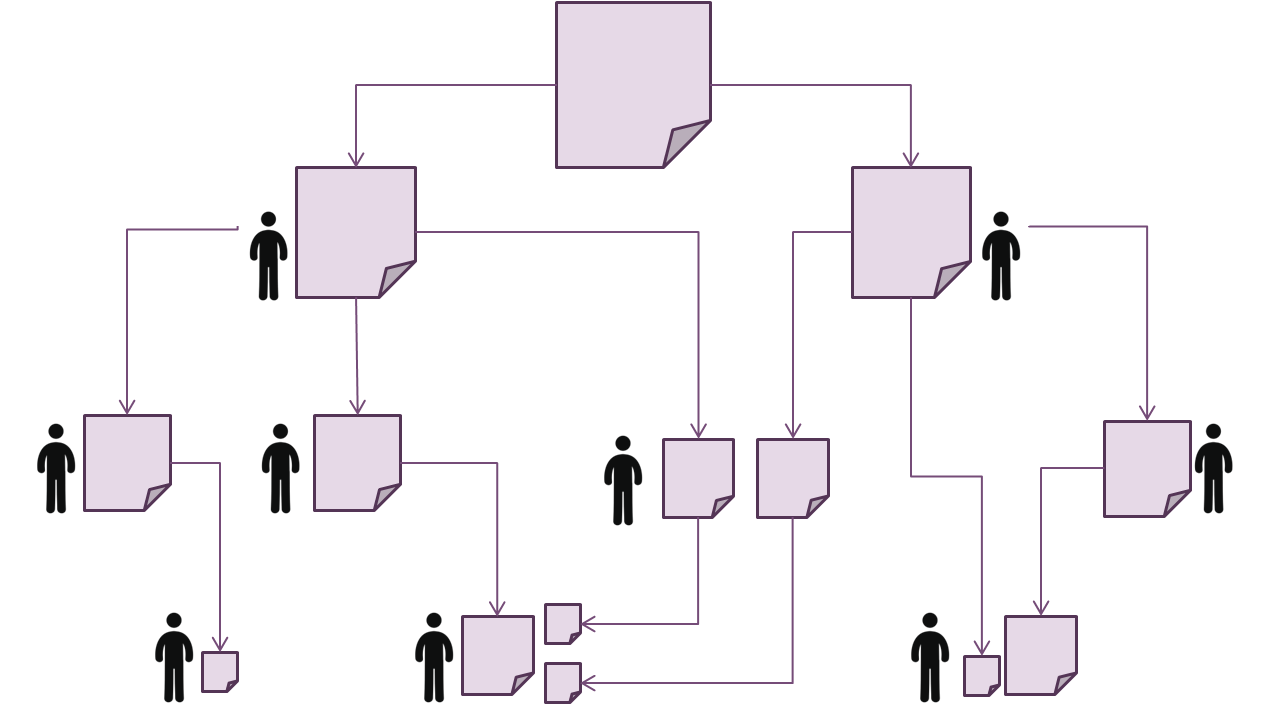
\includegraphics[width=150mm, keepaspectratio]{figures/fileLevel.png}
	\caption{A fájl szintű hozzáférés-szabályozás hátránya}
	\label{fig:fileLevel}
\end{figure}

%----------------------------------------------------------------------------
\subsection{Szabály alapú hozzáférés-szabályozás\protect\footnote{Gabor Bergmann, Csaba Debreceni, Istvan Rath, and Daniel Varro: Query-based Access Control for Secure Collaborative Modeling using Bidirectional Transformations, 2016}}
%----------------------------------------------------------------------------
Az előbbinél hatékonyabb lehet egy szabály alapú hozzáférés-szabályozás, amely során modell szinten, szabályokban fogalmazhatjuk meg, hogy ki milyen olvasási/írási jogosultsággal rendelkezzen a különböző modell elemek felett. Ezen szabályok betartásáért egy ún. lencse felel, ez egy kétirányú modell transzformáció, aminek műveletei a GET és a PUTBACK. Előbbi minden felhasználó számára egy egyedi nézetet készít a modellből, amelyen csak azok a modell elemek (objektumok, attribútumok, referenciák) szerepelnek, amiket a szabályok szerint láthat. A módosítások a PUTBACK művelettel érvényesíthetők, ami előbb ellenőrzi az írási jogosultságokat, és amennyiben azok teljesülnek, végrehajtja a változást, ha nem, akkor visszautasítja a műveletet.

\begin{figure}[!ht]
	\centering
	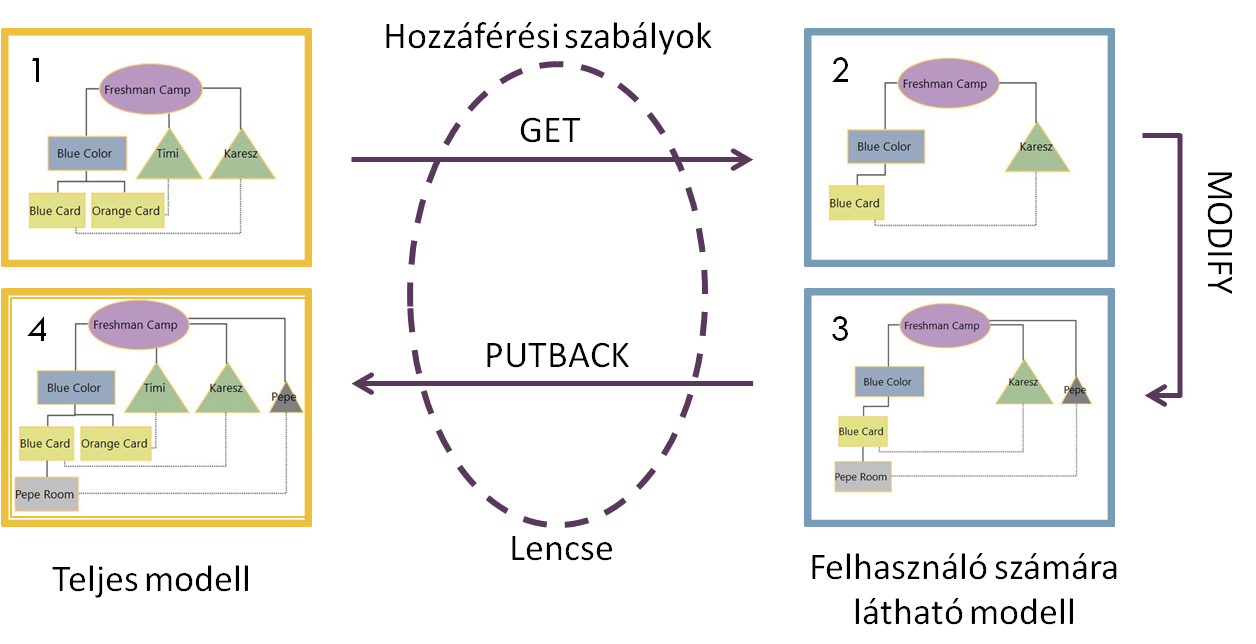
\includegraphics[width=150mm, keepaspectratio]{figures/lens.png}
	\caption{A szabályok betartásáért felelős lencse működése}
	\label{fig:lens}
\end{figure}

\clearpage
%----------------------------------------------------------------------------
\section{MONDO Collaboration Framework}
%----------------------------------------------------------------------------
A MONDO kutatási projekt keretei közt készült egy kollaborációs keretrendszer, amely a másodikként említett szabály alapú hozzáférés-szabályozást alkalmazza. Ennek hiányossága, hogy nem veszi figyelembe az alapértelmezettként megadott hozzáférési szabályokat, valamint az olvasási és írási függőségeket. Az alapértelmezett szabályokat akkor vesszük figyelembe, ha egy modell elemre nincs definiálva egyéb specifikus szabály. Olvasási vagy írási függőségről pedig például akkor beszélünk, amikor egy modell elem látható/módosítható, de az őt tartalmazó elem nem, vagy amikor egy modell elem nem látható, de módosítható. A célom egy olyan, elméletben már létező algoritmus\footnote{Csaba Debreceni, Gábor Bergmann, István Ráth and Dániel Varró: Deriving Effective Permissions for Modeling Artifacts from Fine-grained Access Control Rules, 2016} implementálása, amelynek célja, hogy ezeket a konfliktusokat feloldja.

%----------------------------------------------------------------------------
\chapter{Megismert technológiák}

A következők közül az Eclipse Modeling Framework és Xtext már nem volt számomra teljesen ismeretlen, a témalaboratórium keretei közt foglalkoztam velük.

%----------------------------------------------------------------------------
\section{Eclipse Modeling Framework (EMF)}
%----------------------------------------------------------------------------
Az EMF egy Eclipse pluginekből álló modellező és kódgeneráló keretrendszer. Megkülönbözteti a metamodellt (Ecore modell) a tényleges modelltől, előbbi a modell struktúráját írja le, utóbbi pedig a metamodell konkrét példánya. Az Ecore modell gyakorlatilag osztályokat (EClass), valamint azok attribútumait (EAttribute) és a közöttük lévő referenciákat (EReference) tartalmazza. Az eszköz segítségével Java kódot is generálhatunk a modellünkhöz.

%----------------------------------------------------------------------------
\section{Xtext}
%----------------------------------------------------------------------------
A modellek leírásához modellezési nyelveket használunk. Ezeknek részei az absztrakt szintaxis és a konkrét szintaxisok. Előbbi azt határozza meg, hogy a nyelvnek milyen típusú elemei vannak és ezek milyen kapcsolatban állnak egymással, vagyis ez maga a metamodell. Ehhez több konkrét szintaxis is megadható, ezek olyan szöveges vagy grafikus megjelenítést biztosítanak a modellhez, amiktől olvashatóvá és szerkeszthetővé válik a modell leírása. Az Xtext keretrendszer segítségével szöveges konkrét szintaxis készíthető.

%----------------------------------------------------------------------------
\section{VIATRA Query}
%----------------------------------------------------------------------------
A VIATRA Query egy deklaratív lekérdezési nyelvvel rendelkező modelltranszformációs eszköz. A nyelv segítségével a lekérdezéshez gráfmintákat fogalmazhatunk meg a metamodell osztályaival, attribútumaival, referenciáival, a rendszer pedig azokat a modell elemeket adja vissza, amelyek illeszkednek a megadott mintára.

%----------------------------------------------------------------------------
\chapter{Motivációs példa}
%----------------------------------------------------------------------------
A félévben végzett munkám reprezentálására egy EMF-ben készített, gólyatábor témájú modellt használtam.

%----------------------------------------------------------------------------
\section{Metamodell}
%----------------------------------------------------------------------------
A modell gyökérosztálya maga a tábor, ami tartalmazza a gólya és a senior osztályokat, valamint egymásba ágyazva a „szín” és a „szoba” osztályokat, ezekbe a csoportokba tartoznak a résztvevők. Minden csoport tartalmaz referenciát egy-egy megfelelő típusú seniorra, aki azt irányítja. A seniorok között kétirányú referencia található, a „színseniorok” és a „szobaseniorok” hierarchiájának ábrázolására.

\begin{figure}[H]
	\centering
	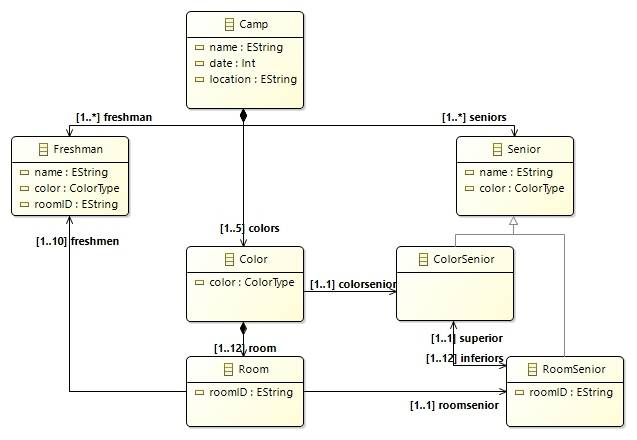
\includegraphics[width=150mm, keepaspectratio]{figures/metamodel.jpg}
	\caption{A gólyatábor metamodellje}
	\label{fig:metamodel}
\end{figure}


%----------------------------------------------------------------------------
\section{Példánymodell}
%----------------------------------------------------------------------------
Az előbbi metamodellnek egy lehetséges példánymodelljében egy kék és egy sárga szín van, mindegyik két-két szobával, valamint a megfelelő típusú senior vezetővel. Ezen a modellen egy hozzáférési szabály lehet a következő: mivel a Zsolti nevű kék színsenior a saját színén belül a szobaseniorok főnöke, ezért azt szerettem volna meghatározni, hogy ő - mint felhasználó - ezekhez az objektumokhoz férjen hozzá és módosíthassa őket.

\begin{figure}[H]
	\centering
	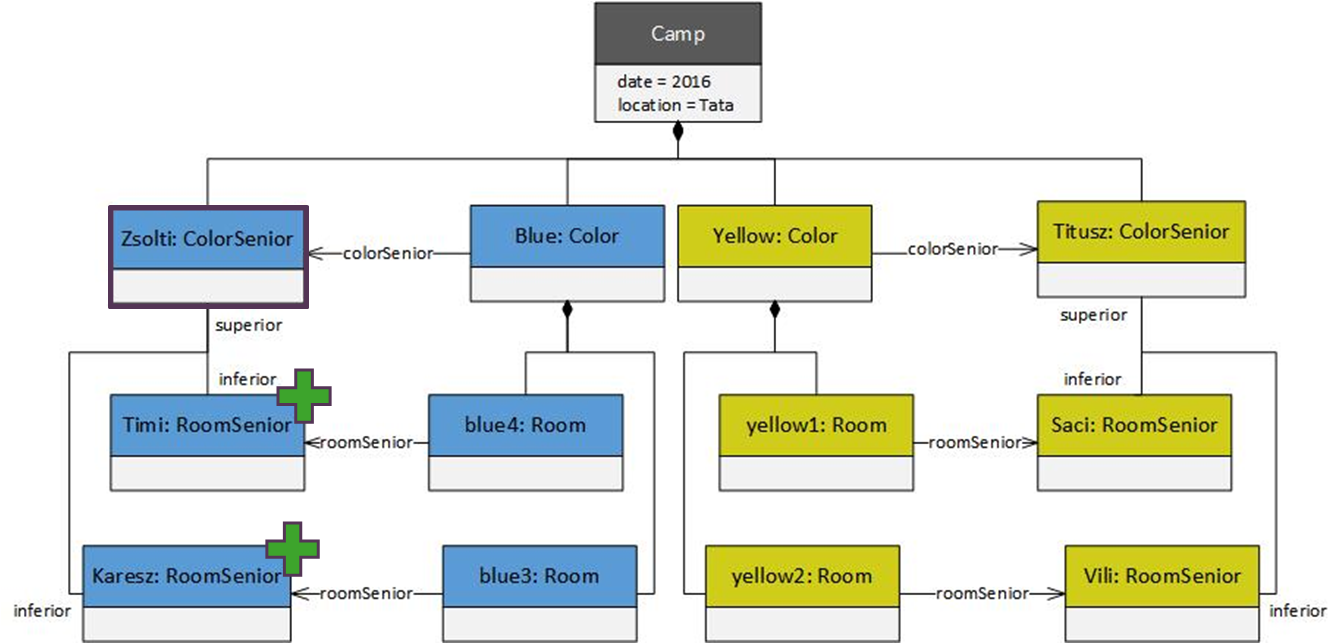
\includegraphics[width=150mm, keepaspectratio]{figures/instance.png}
	\caption{A gólyatábor példánymodellje az érvényesíteni kívánt szabállyal}
	\label{fig:instance}
\end{figure}

%----------------------------------------------------------------------------
\chapter{Hozzáférési szabályok kiértékelése}
%----------------------------------------------------------------------------
A hozzáférési szabályok több elemből állnak. A modell azon részeit, amelyekre a szabály vonatkozik, gráf mintákkal írjuk le. Ezek adják vissza az ún. asseteket, ezek lehetnek objektum (obj), attribútum (attr) vagy referencia (ref) modell elemek, ezekre adhatunk írási vagy olvasási jogosultságokat egyéni felhasználóknak vagy felhasználók egy csoportjának. Ezen kívül pedig prioritást is rendelhetünk a szabályokhoz, ezzel egy fontossági sorrendet felállítva közöttük.

\begin{figure}[H]
	\centering
	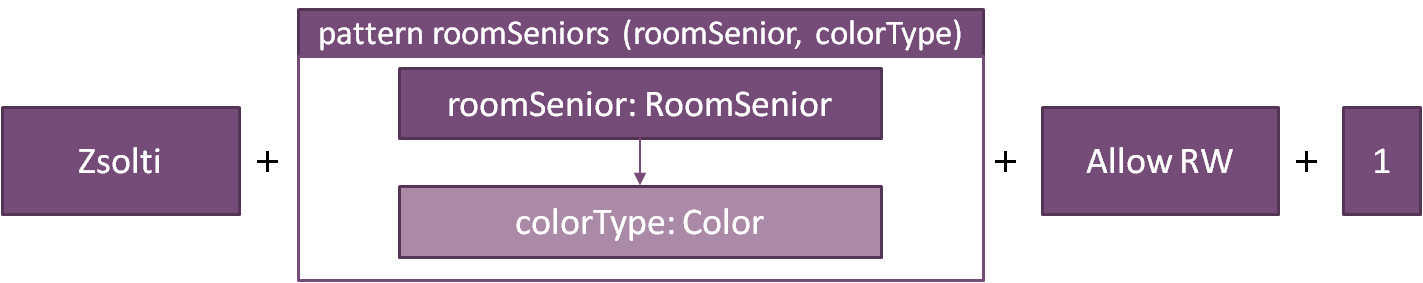
\includegraphics[width=150mm, keepaspectratio]{figures/rule.png}
	\caption{Egy szabály felépítése}
	\label{fig:rule}
\end{figure}

Vagyis a már említett szabályhoz a következőket kell meghatározunk: A Zsolti nevű felhasználónak az adott színű szobasenior objektumokra írási és olvasási engedélyt adunk, 1-es prioritással. Ezzel a gráfmintával egyelőre csak az összes szobaseniort tudjuk lekérdezni a színükkel együtt, később ezt a kört szűkíteni kell még, hogy csak a megfelelő színűek legyenek benne.

A szabályok érvényesítéséhez azokból először ún. judgementeket definiálunk. Egy judgement egy bizonyos asset elérhetőségére vagy módosítására tartalmaz engedélyt vagy tiltást, valamint ennek a prioritását. A hozzáférés-szabályozás ezen judgementek kiértékelése, összevetése alapján dönti el, hogy mely szabályok érvényesülnek. A lenti képen az előbb példaként felhozott szabály alapján létrejövő judgementek láthatók: a Timi és a Karesz nevű objektumok írhatók és olvashatók.

\begin{figure}[H]
	\centering
	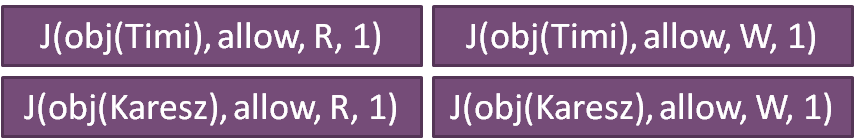
\includegraphics[width=150mm, keepaspectratio]{figures/judgement.png}
	\caption{A létrejövő judgementek}
	\label{fig:judgement}
\end{figure}

A már említett algoritmus - melynek célja a szabályok közötti ütközések feloldása - a megadott szabályok alapján definiált judgementek halmazát alakítja úgy, hogy a közöttük lévő konfliktusokat elemi konfliktusokra vezeti vissza, vagyis egy bizonyos assetre az egyik judgement engedélyez egy bizonyos műveletet, a másik tiltja azt. Ezek feloldásához először a judgementek prioritását veszi figyelembe, ha az megegyezik, akkor pedig az adott szabálynak az engedélyező vagy korlátozó tulajdonságát, amik az allow-t vagy a deny-t teszik dominánsabbá. Továbbá az olvasási/írási függőségek feloldására kibővíti az érvényre jutó judgementek listáját.

%----------------------------------------------------------------------------
\chapter{Nyelvtan}
%----------------------------------------------------------------------------
A szabályok definiálásához először egy Xtext nyelvtant készítettem. Az alábbi ábrán ennek a szöveges szerkesztője látható, amelyben az előbb példaként felhozott szabályt írtam le. Az elején adhatjuk meg a felhasználókat, vagy egy halmazukat, akikre majd a szabályok vonatkoznak. A szabályokat vagyis rule-okat policyba csoportosíthatjuk, erre megszabhatunk egy alapértelmezett jogosultságot (itt az írás/olvasás tiltott), valamint korlátozó vagy engedélyező tulajdonságot, ami megszabja, hogy az azonos prioritású szabályok között a tiltó vagy az engedélyező a dominánsabb. (Itt pl. mivel korlátozó tulajdonságot szabtunk meg, ha lenne még egy szabály, ami a meglévő engedélyezővel szemben a Zsolti nevű felhasználónak megtiltja a hozzáférést ezekhez az objektumokhoz, akkor az a szabály érvényesülne.) A rule elején megadjuk, hogy melyik felhasználóra vonatkozik, és milyen jogokat ad/tilt. (Itt engedélyezzük Zsoltinak az olvasást/írást.) A végén adhatjuk meg hozzá a már említett prioritást. A rule-on belül egy gráflekérdezésre hivatkozunk. (Az én példám szerint ez adja vissza a szobaseniorokat a színükkel együtt.) Ebből választhatunk ki objektum, attribútum vagy referencia asseteket (itt a szobasenior objektumokat), amelyek halmazát különböző megkötésekkel tovább specifikálhatjuk. (A szobaseniorok közül a kékek kellenek).

\begin{lstlisting}
	user Zsolti                                        // Felhasználó(k)                 
	
	policy camp deny RW by default {                   // Alapértelmezett jogosultság
	
	    rule blueRoomSeniors allow RW to Zsolti {      // Jogosultság + felhasználó
	        from query "roomSeniors"                   // Gráflekérdezés
	        select obj(roomSenior)                     // Asset(ek) kiválasztása
	        where colorType is bound to "BlueColor"    // Megkötés(ek)
	    } with 1 priority                              // Prioritás
	
	} with restrictive resolution                      // Korlátozó/engedélyező tulajdonság
\end{lstlisting}

A hozzáférési szabályok definiálását két extra funkció is kényelmesebbé teszi a felhasználó számára. Az egyik az automatikus formázás, a Ctrl+Shift+F billentyűkombinációt lenyomva az alább látható formára alakul a helyesen beírt szöveg. Ezen kívül szintén Java nyelven ScopeProvider-t is írtam, ami pedig Ctrl+space kombinációt a megfelelő helyeken lenyomva egy listából választhatunk az alternatívák közül. Konkrétan a fel-használók, a létező lekérdezések, és a lekérdezés által visszaadott assetek közül válogathatunk.

%----------------------------------------------------------------------------
\chapter{Összefoglalás}
%----------------------------------------------------------------------------
A félév során megismerkedtem a MONDO Collaboration Framework által is megvalósított szabály alapú hozzáférés-szabályozással, annak hiányosságaival, és azt ezt kiegészítő algoritmussal. Megtettem az algoritmus implementálásához szükséges első lépéseket: definiáltam egy Xtext nyelvtant, amellyel meghatározhatók a hozzáférési szabályok, ezt integráltam a meglévő rendszerbe a VIATRA Query technológiával frissítve. A későbbiek folyamán munkám középpontjába az algoritmus implementálását szeretném helyezni.

\end{document}
